\documentclass[mathserif]{beamer}
\usetheme{Luebeck}
%\usepackage[francais]{babel}
\usepackage[utf8]{inputenc} % Uses the utf8 input encoding
\usepackage[T1]{fontenc} % Use 8-bit encoding that has 256 glyphs
\usepackage[style=authoryear,backend=biber]{biblatex}
\addbibresource{main.bib}
\usepackage{etoolbox}
\makeatletter
\patchcmd{\@@description}{\advance\beamer@descdefault by
  \labelsep}{\advance\beamer@descdefault by -1em}{}{}
\makeatother

\usepackage{calc}
\usepackage{xcolor}

\AtBeginSection[]
{
\setbeamercolor{section in toc}{fg=alerted text.fg}
\setbeamercolor{section in toc shaded}{bg=structure!20,fg=structure}
\setbeamertemplate{section in toc shaded}[default][100]
\begin{frame}<beamer>
  \frametitle{Outline}
  \tableofcontents[currentsection,hideallsubsections]
\end{frame}
}

\definecolor{myorange}{RGB}{180,90,0}

\usepackage[nomath]{kpfonts}
\usepackage{eulervm}
%\usepackage{default}

\usepackage{amsthm}
\usepackage{amssymb}
\usepackage{xparse}
\usepackage{thmtools}
\usepackage{stackrel}

%shortcuts
\newcommand{\R}{\mathbb{R}}
\newcommand{\C}{\mathbb{C}}
\newcommand{\Z}{\mathbb{Z}}
\newcommand{\N}{\mathbb{N}}
\newcommand{\fii}{\varphi}
\newcommand{\dd}{\mathrm{d}}
\newcommand{\CP}{\mathbb{CP}}
\renewcommand{\S}{\mathbb{S}}
\DeclareMathOperator{\Sp}{Sp}
\DeclareMathOperator{\tr}{tr}
\DeclareMathOperator{\dist}{dist}

% theorems configuration

\makeatletter
\newtheoremstyle{indented}
{7pt} %vertical space before
{7pt} % vertical space after
{} %{\addtolength{\@totalleftmargin}{2.5em}
	%\addtolength{\linewidth}{-3.5em}
	%\parshape 1 3.5em \linewidth} %body font
{1.5em} %indent
{\bfseries} %header font
{.} %punctuation
{.5em} %horizontal space after header
{} %header specification

\theoremstyle{definition}

\newtheorem{defn}{Définition}[section]

\theoremstyle{plain}
%\newtheorem*{theorem*}{Theorem}

\newtheorem{thm}{Théorème}

\renewcommand{\thetheorem}{\Alph{theorem}}
\newenvironment{preuve}{
	\noindent \textbf{Proof. }}{\hfill $\square$\medskip\par}

\newtheorem{exemple}[defn]{Example}
\newtheorem{prop}[defn]{Proposition}
\newtheorem{corr}[defn]{Corollary}
\newtheorem{por}[defn]{Porisme}
\newtheorem{ex}[defn]{Example}
\newtheorem{lem}[defn]{Lemma}
\newtheorem{conj}{Conjecture}
\newtheorem{ax}{Axiom}  %Axioms have their own numerotation

\theoremstyle{definition}
\newtheorem{rem}[defn]{Remark} %remarks are not indented
\newtheorem{rems}[defn]{Remarks}

%--------------
% Mise en page mathématique
%--------------
\addtolength{\jot}{.2em}


\title{Low-energy spectrum of Toeplitz operators}
\author[Alix Deleporte]{Alix Deleporte\\Advisor: Nalini Anantharaman}
\institute[IRMA]{Institut de Recherche Mathématique
  Avancée\\Université de Strasbourg}
\titlegraphic{
\includegraphics[height=0.8cm]{logoIRMA.pdf}\hfill
\includegraphics[height=0.8cm]{logounistra.pdf}\hfill
\includegraphics[height=0.8cm]{logoCNRS.pdf}\hfill
\includegraphics[height=0.7cm]{ANR.png}\hfill
\includegraphics[height=0.8cm]{logoENS.jpg}}

\newcommand{\spline}{\hline}
\renewcommand{\arraystretch}{1.3}

\DeclareSourcemap{
  \maps[datatype=bibtex]{
    \map[overwrite=true]{
      \step[fieldsource=author,
            match=Deleporte,
            final]
      \step[fieldset=keywords, fieldvalue=Deleporte]
    }
  }
}
\begin{document}

\beamertemplatenavigationsymbolsempty

    \expandafter\def\expandafter\insertshorttitle\expandafter{%
       \insertshorttitle\hfill%
       \insertframenumber}


\begin{frame}
	\titlepage
\end{frame}

\begin{frame}
  \frametitle{Introduction}
  \begin{itemize}
  \item<1-> {\bfseries spin systems}: models for magnetism in solids.
  \item<2-> {\bfseries classical spins}: one atom at site $i$
    $\rightsquigarrow$ one spin $s_i\in \S^2$.
  \item<3> Heisenberg antiferromagnet: Graph $G=(V,E)$,
    
    search the minima of the following energy:
    \[
      (s_i)_{i\in V}\mapsto\sum_{i\sim j}s_i\cdot s_j.
    \]
    Here $i\sim j$ when the atoms $i$ and $j$ are neighbours in $G$
    and $\cdot$ is the scalar product.
  \end{itemize}
\end{frame}

             \begin{frame}
         \frametitle{Introduction}
   \begin{center}
     \begin{picture}(50,50)
           \only<1>{\put(-125,-80){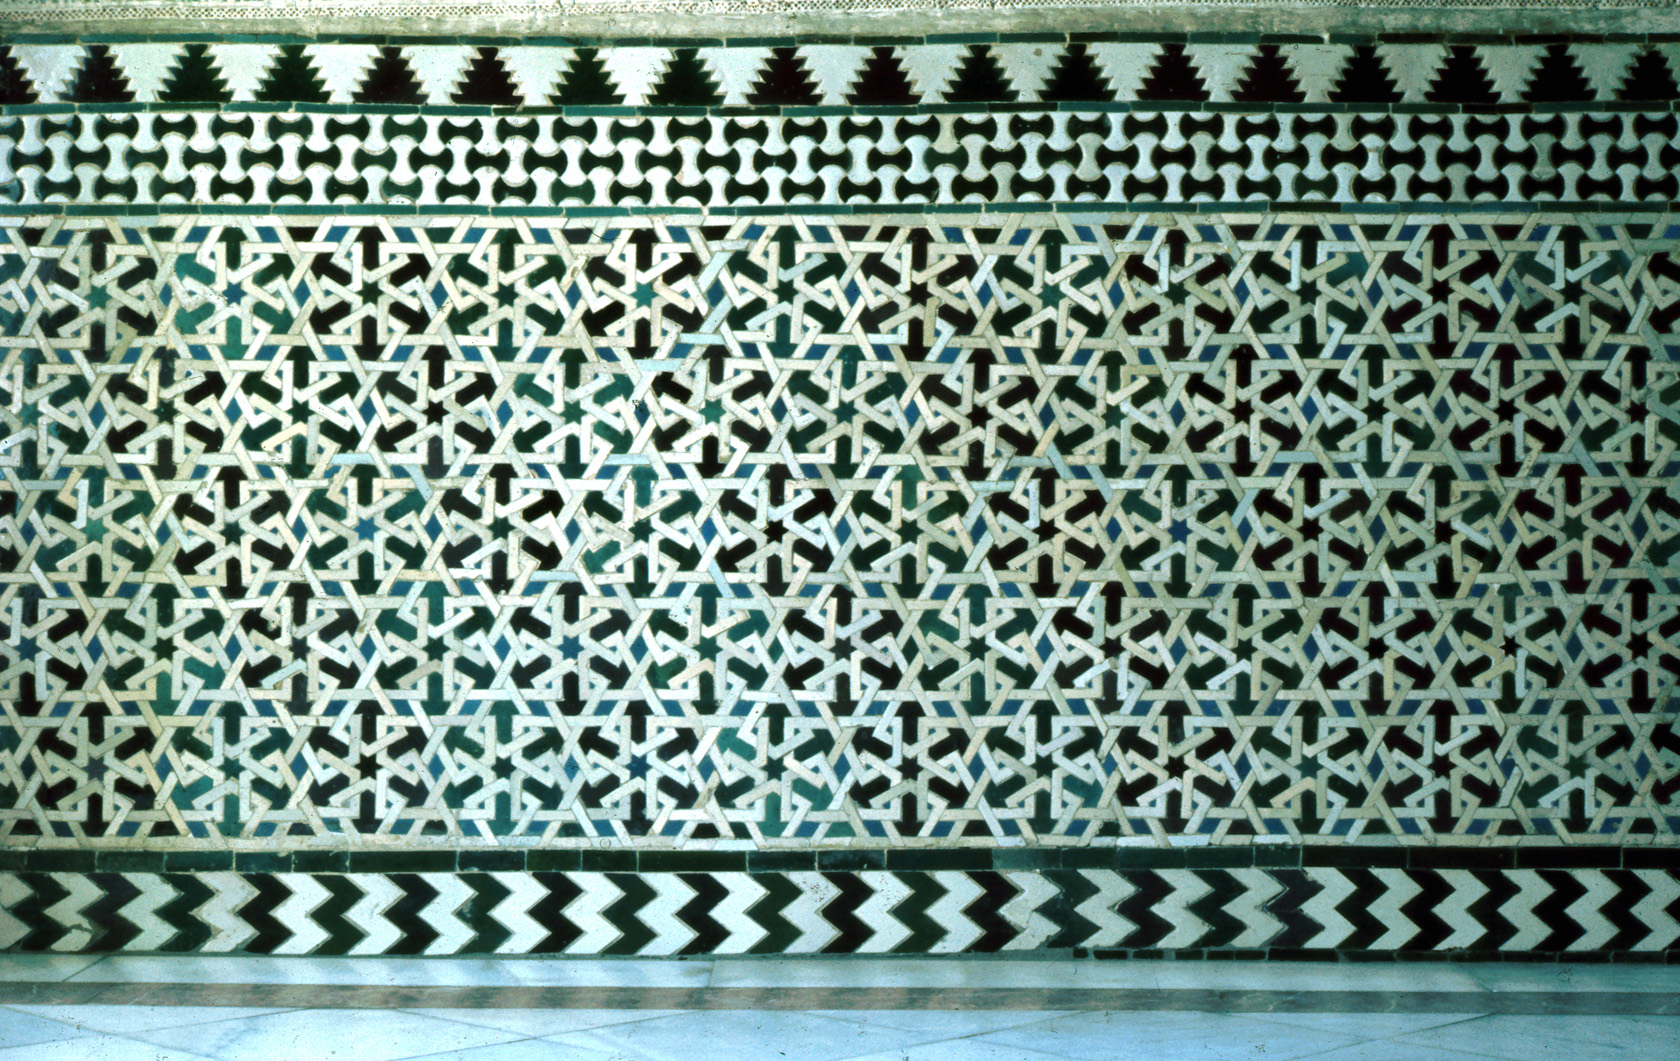
\includegraphics[scale=9]{Alcazar.png}}}
           \only<2>{\put(-125,-80){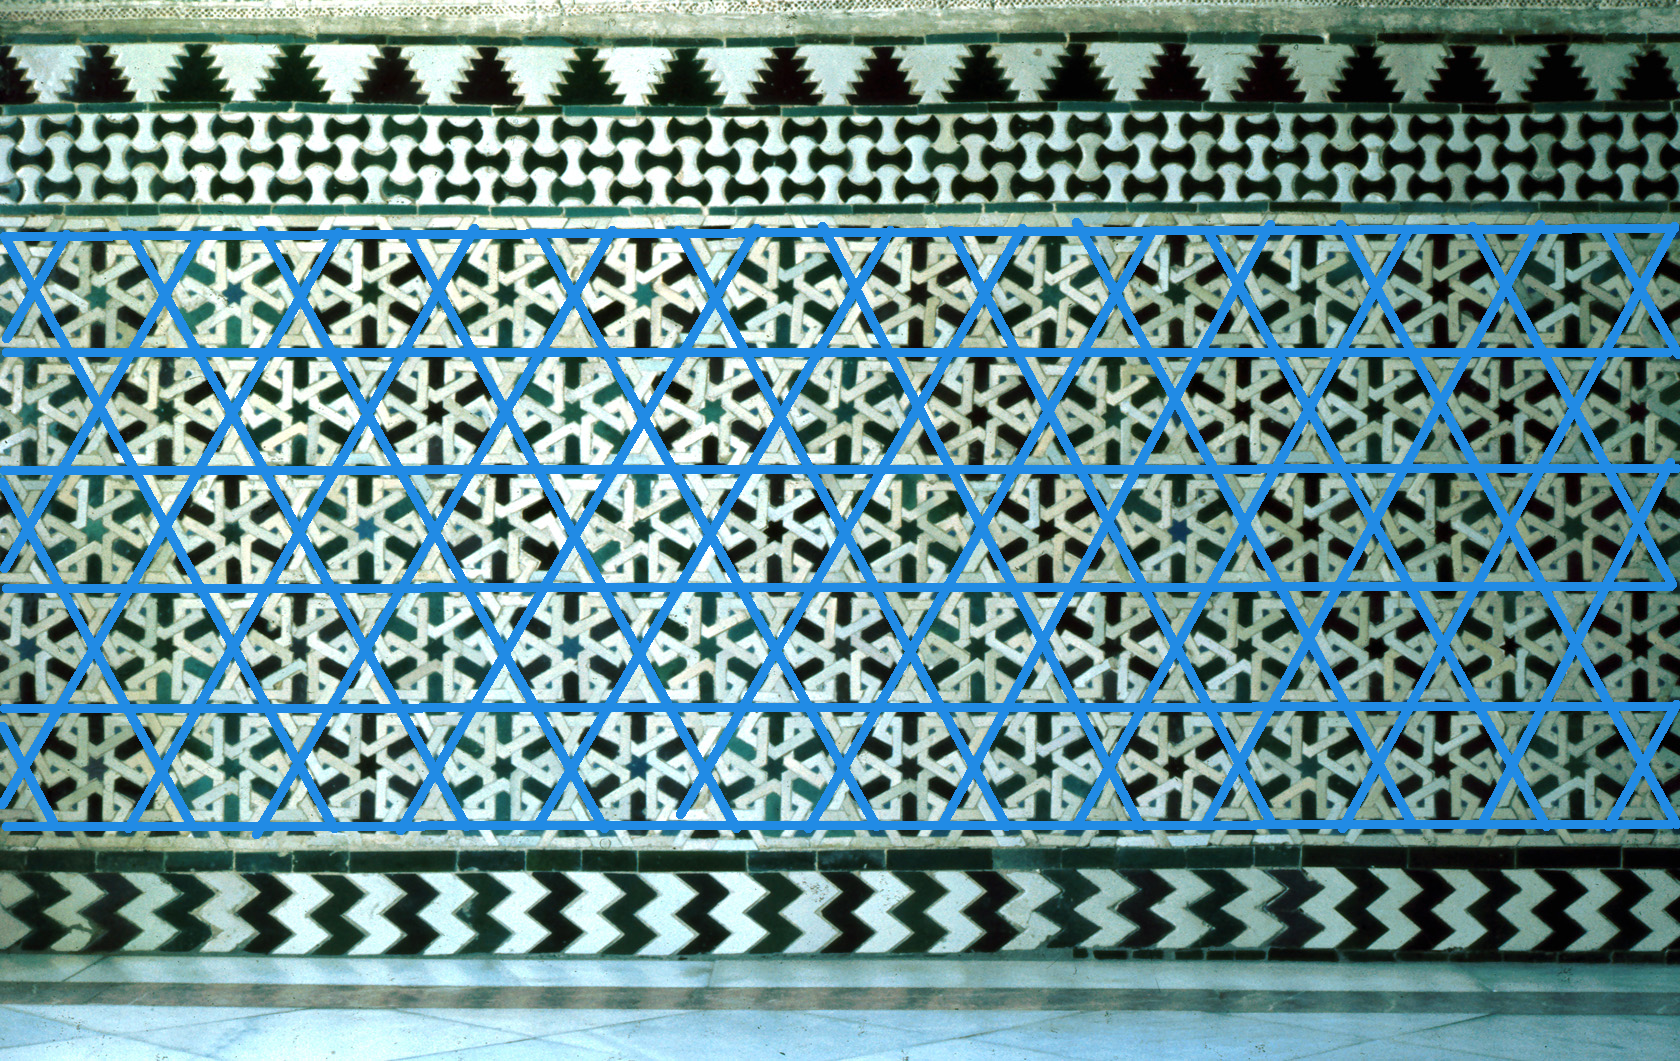
\includegraphics[scale=9]{Alcazar-Kagome.png}}}
           \only<3>{\put(-112,-80){\includegraphics[scale=0.32]{kagome-svg.png}}}
           \only<4>{\put(-112,-80){\includegraphics[scale=0.32]{kagome-spins-svg.png}}}
           \only<5>{\put(-112,-80){\includegraphics[scale=0.32]{kagome-spins-2-svg.png}}}
         \end{picture}
       \end{center}
     \end{frame}

% \begin{frame}
%   \frametitle{Introduction}
%   \begin{center}
%     \begin{picture}(50,50)
%       \put(-125,-80){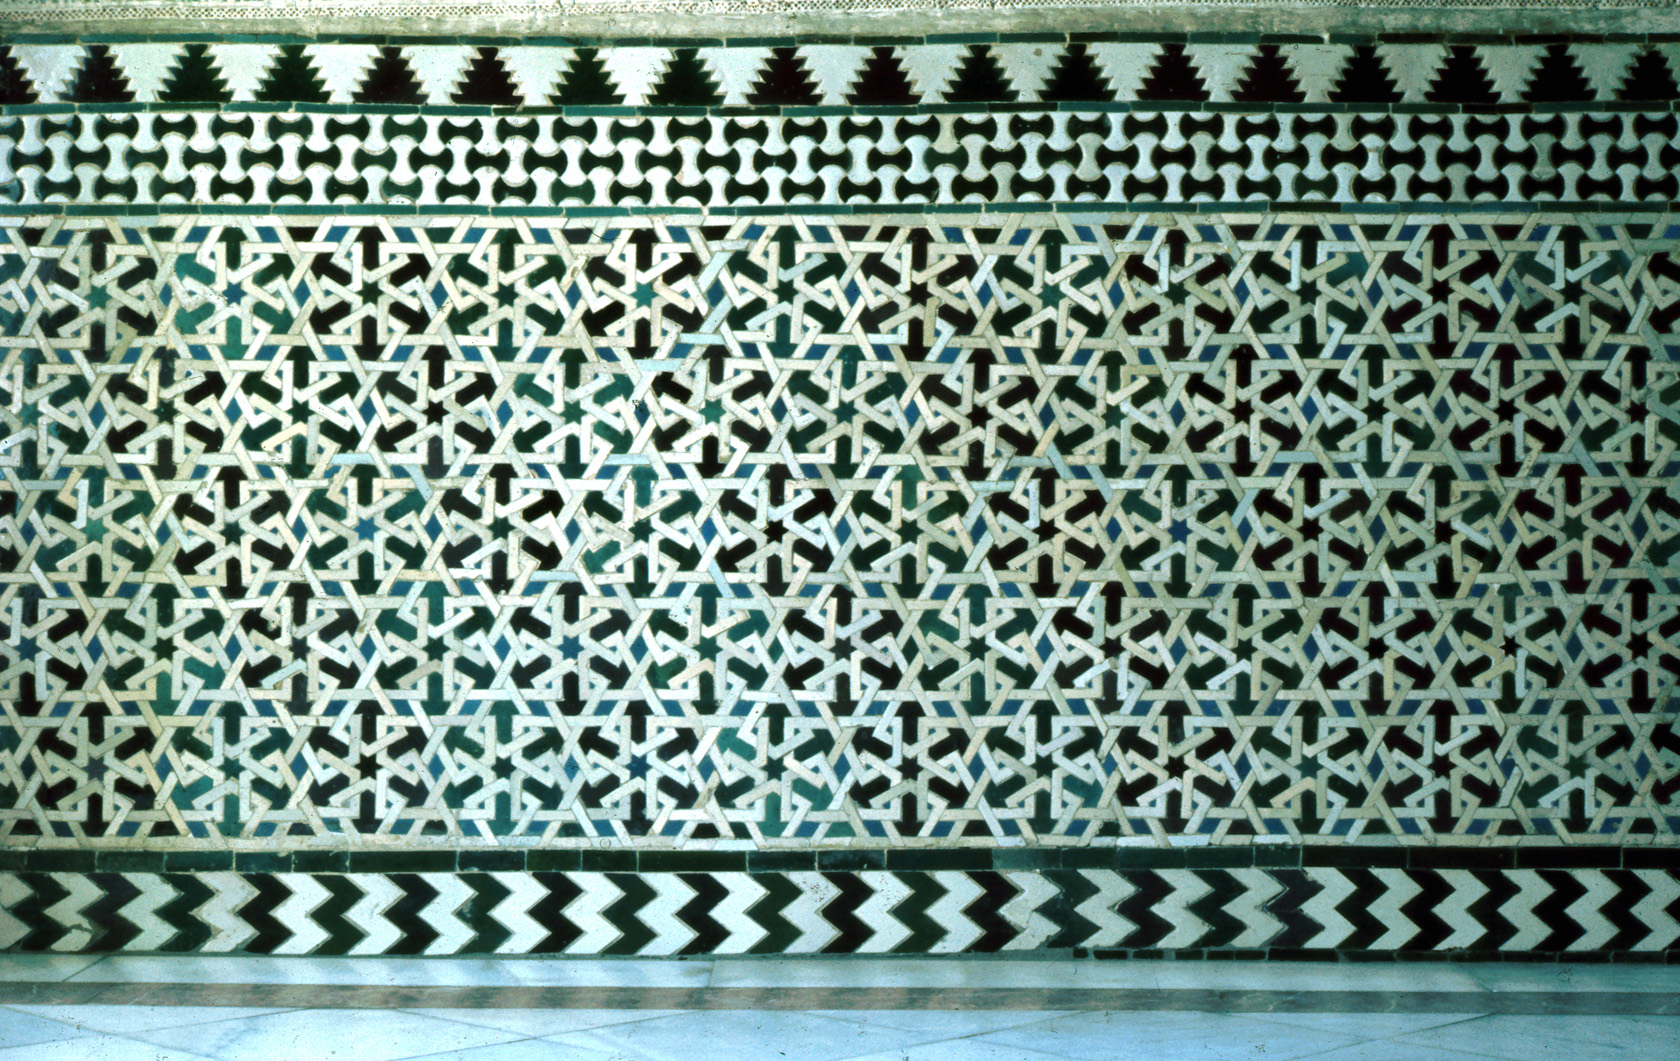
\includegraphics[scale=9]{Alcazar.png}}
%     \end{picture}
%   \end{center}
% \end{frame}

% \begin{frame}
%   \frametitle{Introduction}
%   \addtocounter{framenumber}{-1}
%   \begin{center}
%     \begin{picture}(50,50)
%       \put(-125,-80){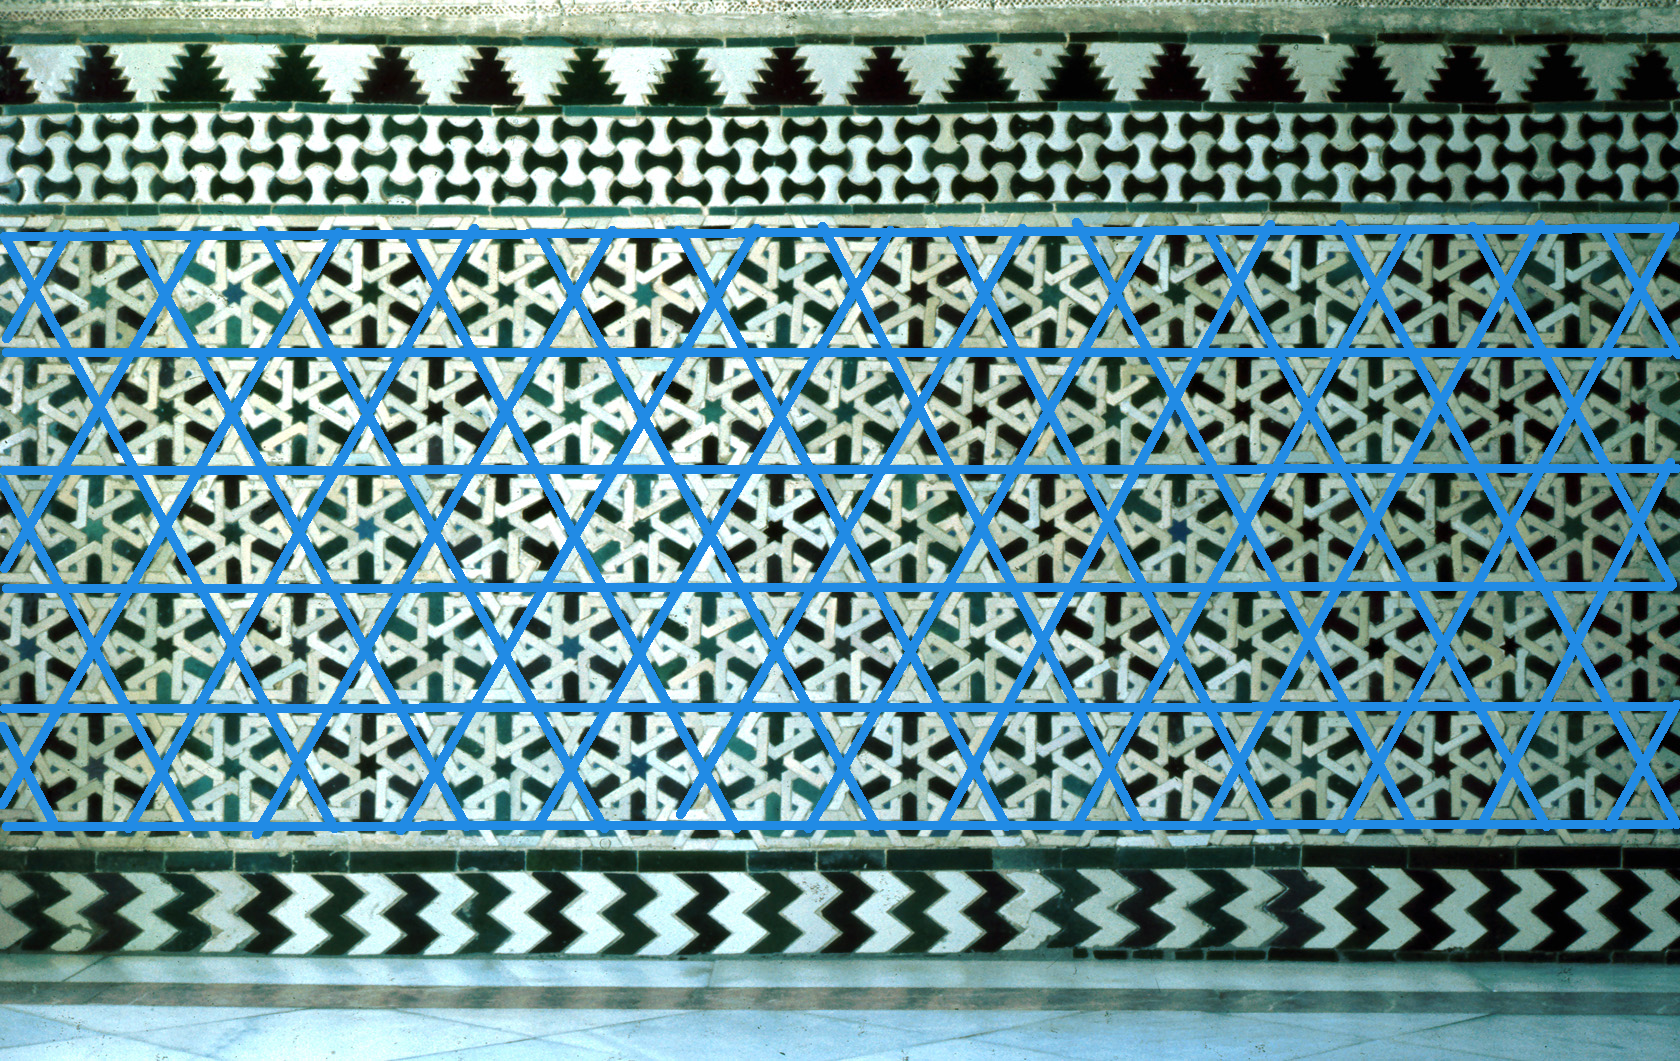
\includegraphics[scale=9]{Alcazar-Kagome.png}}
%     \end{picture}
%   \end{center}
% \end{frame}

% \begin{frame}
%   \frametitle{Introduction}
%   \addtocounter{framenumber}{-1}
%   \begin{center}
%     \begin{picture}(50,50)
%       \put(-112,-80){\includegraphics[scale=0.32]{kagome-svg.png}}
%     \end{picture}
%   \end{center}
% \end{frame}

% \begin{frame}
%   \frametitle{Introduction}
%   \addtocounter{framenumber}{-1}
%   \begin{center}
%     \begin{picture}(50,50)
%       \put(-112,-80){\includegraphics[scale=0.32]{kagome-spins-svg.png}}
%     \end{picture}
%   \end{center}
% \end{frame}

% \begin{frame}
%   \frametitle{Introduction}
%   \addtocounter{framenumber}{-1}
%   \begin{center}
%     \begin{picture}(50,50)
%       \put(-112,-80){\includegraphics[scale=0.32]{kagome-spins-2-svg.png}}
%     \end{picture}
%   \end{center}
% \end{frame}





    \begin{frame}\frametitle{Introduction}
	\begin{itemize}
		\item Quantum spin: self-adjoint matrices
                  $S_x,S_y,S_z\in M_{N+1}(\C)$ \[[S_x,S_y]=\frac{2i}{N}S_z\qquad
                    [S_y,S_z]=\frac{2i}{N}S_x\qquad [S_z,S_x]=\frac{2i}{N}S_y.\]
                \item Several spins $\rightarrow$ {\color{myorange} tensor product}.
                    \[S_{x,i}=\underbrace{Id\otimes \cdots\otimes Id}_{i-1}\otimes S_x\otimes
                                                                              \underbrace{Id\otimes
                                                                                \cdots
                                                                              \otimes
                                                                              Id}_{d-i}.\]
                                                                          
                                                                        \item<2>
                                                                          Quantum
                                                                          energy
                                                                          (matrix
                                                                          of
                                                                          size
                                                                          $(N+1)^d$):
                                                                          \[
                                                                            \sum_{i\sim j}S_{i,x}S_{j,x}+S_{i,y}S_{j,y}+S_{i,z}S_{j,z}.\]
                    
      
      \end{itemize}
    \end{frame}
    \begin{frame}
      \frametitle{Introduction}
      Quantum energy is a self-adjoint matrix $\Rightarrow$
      
      \hspace{1em}eigenvalues
      $\lambda_1\leq \lambda_2\leq \cdots\leq \lambda_{(N+1)^d}$

      \hspace{1em}and associated eigenvectors.
      
      Goal: qualitative study of eigenvectors associated with
      $\lambda_1$ (ground states) or other small eigenvalues.
      
      \hfill
      
      \uncover<2>{Physics claim: {\color{myorange} quantum-classical
          correspondence} as $N\to +\infty$.
        
        \hfill
        
      Prediction [DS98]: lowest-energy eigenvectors concentrate on {\color{myorange} some} classical configurations.}
    \end{frame}
      \begin{frame}
        \frametitle{Introduction}
        Toeplitz quantization:
        \begin{itemize}
          \item treat $N\to +\infty$ as a semiclassical
       limit
     \item see eigenvectors above as sections over $(\S^2)^d$.
     \end{itemize}
     \uncover<2->{Questions:}
     \begin{itemize}
        \item<2-> Where does the ground state concentrate?
        \item<3> What is the decay speed outside the concentration set?
        \end{itemize}
      \end{frame}

      \begin{frame}
        \frametitle{Introduction}
        \setbeamercovered{transparent}
        {\footnotesize
        \begin{description}
        \item<1>[{[Del19]}] Alix Deleporte. “Low-Energy Spectrum of Toeplitz Operators: The Case
of Wells.” In: Journal of Spectral Theory 9 (2019).
\item<1-2> [{[Del17++]}] Alix Deleporte. “Low-Energy Spectrum of Toeplitz Operators with a
Miniwell.” In: arXiv 1610.05902 (2017).
\item<1>[{[Del18a++]}] Alix Deleporte. “Quantum Selection for Spin Systems.” In: arXiv
1808.00718 (2018).
\item<1>[{[Del18b++]}] Alix Deleporte. “The Bergman Kernel in Constant Curvature.” In:
arXiv 1812.06648 (2018).
\item<1-2>[{[Del18c++]}] Alix Deleporte. “Toeplitz Operators with Analytic Symbols.” In: arXiv
1812.07202 (2018).
\item<1>[{[Del19++]}] Alix Deleporte. “WKB Eigenmode Construction for Analytic Toeplitz
  Operators.” In: arXiv 1901.07215 (2019).
        \end{description}}
      \end{frame}

      



      \section{Toeplitz operators}

\subsection{Construction}
\begin{frame}
  \frametitle{Setting}
  \begin{itemize}
  \item Compact, complex, symplectic manifold $M$
    under compatibility conditions (K\"ahler, quantizable).
    \item<2-> There exists a natural complex line bundle $L$ over $M$.
\uncover<3->{\item Quantum space $H_N(M)$ of holomorphic sections of
  $L^{\otimes N}$ (Remark: holomorphic functions are constant).}
\uncover<4->{\item Szeg\H{o} projector $S_N:L^2(M,L^{\otimes N})\to H_N(M).$}
  \end{itemize}
  \uncover<5>{The Szeg\H{o} projector has an integral kernel (section
    over $M^2$):
    \[
      (S_Nu)(x)=\int_M S_N(x,y)u(y) \omega^{\wedge d}(dy).
    \]
    }
\end{frame}


\begin{frame}
  \frametitle{Toeplitz quantization}
  Let $f\in L^{\infty}(M,\C)$. The Toeplitz operator associated
  with $f$ is the bounded operator
\begin{center}
\begin{array}{rcl}
 		T_N(f):H_N(M)&\to & H_N(M)\\
		u& \mapsto& \only<1>{fu}\only<2->{S_N(fu)}.
 		\end{array}
\end{center}
\uncover<3->{Correspondence with pseudodifferential operators when $M$
  is replaced with $\C^n$.}
\uncover<4>{Advantages:
\begin{itemize}
\item If $f\geq 0$ then $T_N(f)\geq 0$.
\item Quantum states are sections over the {\color{myorange} whole manifold} M.
\end{itemize}}
\end{frame}

\subsection{Case of the sphere}

\begin{frame}
  \frametitle{Case $M=\S^2$}
  Stereographic chart: $L$ is topologically trivial.

  \hspace{9.5em}Its hermitian metric is
  $\frac{1}{1+|z|^2}|\cdot|^2.$ \[H_N(M)\simeq \left\{f\text{ holo on $
        \C$},\,\int_{\C}\cfrac{|f|^2}{(1+|z|^2)^{N+2}}<\infty\right\}=\C_N[X].\]
 \uncover<2->{Expression of the Szeg\H{o}
 kernel in this chart:\[S_N(z,w)=\cfrac{N+1}{\pi}\left(\cfrac{1+z\overline{w}}{\sqrt{(1+|z|^2)(1+|w|^2)}}\right)^N.\]}
\uncover<3->{
  \only<3>{\[T_N(\text{base coords})=\vphantom{\frac{N-2}{N}}\text{spin matrices}.\]}
  \only<4>{\[T_N(\S^2\ni (x,y,z)\mapsto x)=\frac{N-2}{N}S_x.\]}
  }
\end{frame}

\subsection{Semiclassical limit}
\begin{frame}
  \frametitle{The Szeg\H{o} kernel}
 On $\S^2$, there holds $S_N(x,y)=(N+1)\Psi^{\otimes
      N}(x,y)$, where $\Psi$ is a fixed section over $M\times M$.
    \uncover<2->{\begin{theorem}[{[Cha03]}]
        Let $M$ be a compact, quantizable almost K\"ahler manifold. There exists a section
        $\Psi$ and a sequence of functions $(s_k)_{k\geq 0}$ on
        $M\times M$ such that, uniformly in $(x,y)\in M^2$,
      \[
        S_N(x,y)=N^d\Psi^{\otimes
          N}(x,y)(s_0+N^{-1}s_1+\cdots)(x,y)+O(N^{-\infty}).
      \]
      Here, for some $c>0$,
      \[
        |\Psi(x,y)|\leq e^{-c\dist(x,y)^2}.
        \]
      \end{theorem}
    \uncover<3>{Meaning: we can sum up to $N^{-K}$ and have $O(N^{-K-1})$ error.}}
    
\end{frame}


\begin{frame}
  \frametitle{Approaches for kernel estimates}
    \begin{itemize}
    \item FIOs with complex phase [SZ02, Cha03]: versions of
      the result above, remainder $O(N^{-\infty})$.
    \item Elliptic (weighted) estimates on $-\Delta$ [MM07, Kor17++]:
      generalisations to other geometries (spin$^c$-Dirac, Bochner).
    \item Partial Bergman kernels [HLX17++]: if $M$ is {\color{myorange}
        real-analytic}, the remainder is $O(e^{-c\sqrt{N}})$ with
      $c>0$.
    \item New analytic calculus [Del18c++,RSV18++]: if $M$ is
      {\color{myorange} real-analytic},
      the remainder is $O(e^{-cN})$ with $c>0$.
    \end{itemize}
  \end{frame}

  \begin{frame}
    \frametitle{Calculus of Toeplitz operators}
    Asymptotics of the Szeg\H{o} kernel $\rightarrow$ composition and
    inversion of Toeplitz operators assocaited with smooth
    functions.

    \begin{theorem}[{[Cha03]}]Let $M$ be smooth. Let $a$ and $b$ be
      smooth real-valued functions on $M$. Then there exists a sequence $(c_k)_{k\geq
        0}\in (C^{\infty}(M,\R))^{\N}$ such that
      \[
        T_N(a)T_N(b)=T_N(c_0+N^{-1}c_1+\cdots)+O(N^{-\infty}).
        \]

        If $a$ does not vanish, then there exists a sequence
        $(d_k)_{k\geq 0}\in (C^{\infty}(M,\R))^{\N}$ such that
        \[
          T_N(a)T_N(d_0+N^{-1}d_1+\cdots)=S_N+O(N^{-\infty}).
          \]
    \end{theorem}
  \end{frame}

  \subsection{Analytic regularity}
  
\begin{frame}
  \frametitle{New symbol classes in real-analytic regularity}

  Let $a$ be an analytic function on an analytic manifold $X$. $\exists C_a,r>0, \forall
  j\in \N, \|a\|_{C^j(X)}\leq C_ar^jj!$.
\uncover<2->{
  \begin{defn}[{[Del18c++]}]
    Let $X$ be an analytic manifold with boundary.

    For parameters $r,R,m\in (\R^+_*)^3$, we define the space
    $S^{r,R}_m(X)$ as the set of sequences $a=(a_k)_{k\geq 0}$ of
    real-analytic functions on $X$ such that, for some $C_a>0$, for
    all $j,k\in \N$,
    \[
      \|a_k\|_{C^j(X)}\leq
      C_ar^jR^k(j+k)!\only<2>{(1+j+k)^{-m}\vphantom{\underbrace{(1+j+k)^{-m}}_{\text{new
          (with respect to [Sjö82])}}}}\only<3->{\underbrace{(1+j+k)^{-m}}_{\text{new
          (w.r.t. [Sjö82])}}}.\]
  \end{defn}

}
\uncover<3->{
   $S^{r,R}_m(X)$ behaves better with respect to standard manipulations (product,
    inversion, stationary phase lemma) than $S^{r,R}_0(X)$.
  }
\end{frame}
\begin{frame}
  \frametitle{Calculus of covariant Toeplitz operators}
Let $U$ be a neighbourhood of the diagonal in $M\times M$. Let $a=(a_k)_{k\in \N}\in S^{r,R}_m(U)$ be a sequence of holomorphic
  functions on $U$. We define
  \[
    T_N^{cov}(a)(x,y)=N^d\Psi^{\otimes
      N}(x,y)(a_0+N^{-1}a_1+\cdots)(x,y){+\color{myorange} O(e^{-cN})}.
  \]
  \vspace{-1em}
  \uncover<2>{
  \begin{theorem}[{[Del18c++]}]
    Let $M$ be real-analytic. Let $a\in S^{r,R}_m(U)$ and $b\in
    S^{2r,2R}_m(U)$ with $U$ as above. Then there exist
    $a\sharp b\in S^{2r,2R}_m(U)$ and $c>0$ such that
    \[T_N^{cov}(a)T_N^{cov}(b)=T_N^{cov}(a\sharp b)+O(e^{-cN})\]

    When $a$ is nonvanishing, from $a\sharp b$ one can recover $b$ .
  \end{theorem}
 $\Rightarrow \; S_N=T_N^{cov}(s)+O(e^{-cN})$
for some analytic symbol $s$.
}
\end{frame}

\section{Localisation of low-energy states}

\subsection{Localisation at the classical minimal set}
\begin{frame}
  \frametitle{Speed of localisation}
 For $N\in \N$, let $u_N$ be a normalised eigenvector associated with
 the smallest eigenvalue of $T_N(f)$. Let $Z=\mathop{argmin}(f)$.
  \begin{theorem}[{[Cha00]}]
  If f is {\color{myorange}smooth} and $U\subset M$ is at positive distance from $Z$, then \[\int_{U}|u_N|^2=O(N^{-\infty}).\]\vspace{-1.2em}
\end{theorem}
\uncover<2>{
\begin{theorem}[{[Del18c++]}]
If f is {\color{myorange}real-analytic} and $U$ is as above, there exists $c>0$ such that
      \[
        \int_{U}|u_N|^2=O(e^{-cN}).\vspace{-0.5em}
      \]
    \end{theorem}}
\end{frame}



\subsection{Subprincipal effects on localisation}
\begin{frame}
  \frametitle{Characteristic value}
  \begin{itemize}
  \item Let $f$ be smooth and $Z$ be as above. One can construct a continuous function $\mu$ on $Z$, which only depends on the Hessian of $f$.
    \item $\mu(x)$ measures the contributions of order $N^{-1}$ in the quantum
    energy near $x$.
  \item<2-> {\color{myorange} Quantum selection}: the ground states of $T_N(f)$
    concentrate only on the subset $Z_{\mu}$ of $Z$ where also $\mu$ is minimal.
  \end{itemize}
  
  \uncover<3>{\begin{description}
    \item[{{\color{white} blaa\hspace{3pt}a}[HS86]}] case of a Schrödinger operator $-\hbar^2\Delta+V$, where\vspace{-1.2em}
      \begin{itemize}
      \item $V$ vanishes on a smooth submanifold $Z$
      \item Its transverse Hessian is nondegenerate on $Z$.
      \end{itemize}
    \item[{[HM96,HK09]}] case of a magnetic Schrödinger operator with similar conditions.
    \end{description}
    }

\end{frame}

\begin{frame}
  \frametitle{Subprincipal localisation}
  \begin{theorem}[{[Del17++]}]
    Let $M$ be smooth, let $f\in C^{\infty}(M,\R)$ and let $Z_{\mu}$ and
    $(u_N)_{N\geq 0}$ be as above.

    For all $U\subset M$ at positive distance from $Z_{\mu}$, one has
    \[
      \int_U
      |u_N|^2=O(N^{-\infty}).
      \]
  \end{theorem}
\end{frame}

\begin{frame}
  \frametitle{Particular case: spin systems}
  \begin{itemize}
\item  Framework: fixed number of particles $d$ , spin parameter $N$ tends to infinity.

  \item<2->{Computations for this particular case
    $M=(\S^2)^d$ [Del18b++].}

  \item<3>{{\color{myorange} Open problem}: where is $\mu$ minimal among classical
      configurations on the Kagome lattice?}
  \end{itemize}
\end{frame}

     \begin{frame}
        \frametitle{Publications}
        {\footnotesize
        \begin{description}
        \item[{[Del19]}] Alix Deleporte. “Low-Energy Spectrum of Toeplitz Operators: The Case
of Wells.” In: Journal of Spectral Theory 9 (2019).
\item[{[Del17++]}] Alix Deleporte. “Low-Energy Spectrum of Toeplitz Operators with a
Miniwell.” In: arXiv 1610.05902 (2017).
\item[{[Del18a++]}] Alix Deleporte. “Quantum Selection for Spin Systems.” In: arXiv
1808.00718 (2018).
\item[{[Del18b++]}] Alix Deleporte. “The Bergman Kernel in Constant Curvature.” In:
arXiv 1812.06648 (2018).
\item[{[Del18c++]}] Alix Deleporte. “Toeplitz Operators with Analytic Symbols.” In: arXiv
1812.07202 (2018).
\item[{[Del19++]}] Alix Deleporte. “WKB Eigenmode Construction for Analytic Toeplitz
  Operators.” In: arXiv 1901.07215 (2019).
        \end{description}}
      \end{frame}

\subsection{Future work}
\begin{frame}
  \frametitle{Perspectives}
    \begin{itemize}
    \item Low-energy time evolution.
    \item Large number of sites: $\stackrel[d\to +\infty]{}{\lim}\stackrel[N\to +\infty]{}{\lim}\stackrel{?}{=}\stackrel[N\to +\infty]{}{\lim}\stackrel[d\to +\infty]{}{\lim}$.
    \item Exponential decay in quantum selection.
    \item Non self-adjoint operators.
    \end{itemize}
  \end{frame}

  \begin{frame}
    \frametitle{Thanks}
    \centering 
    {\Large Thanks for your attention!}
  \end{frame}
  

  \begin{frame}[allowframebreaks]
    \frametitle{Bibliography}
        {\footnotesize
        \begin{description}
        \item[{[Cha00]}] Laurent Charles. “Aspects Semi-Classiques de La Quantification Géométrique.” PhD thesis. Université Paris 9, 2000.
        \item[{[Cha03]}] Laurent Charles. “Berezin-Toeplitz Operators, a Semi-Classical Approach.” en. In: Communications in Mathematical Physics 239.1-2
(Aug. 2003), pp. 1–28.
        \item[{[DS98]}] Benoît Douçot and Patrice Simon. “A Semiclassical Analysis of Order
from Disorder.” en. In: Journal of Physics A: Mathematical and General
31.28 (1998), p. 5855.
\item[{[HK09]}] Bernard Helffer and Yuri A. Kordyukov. “Semiclassical Analysis of
Schrödinger Operators with Magnetic Wells.” In: Contemporary Mathematics 500 (2009), p. 105.
\item[{[HM96]}] Bernard Helffer and Abderemane Mohamed. “Semiclassical Analysis for
the Ground State Energy of a Schrödinger Operator with Magnetic
Wells.” In: Journal of Functional Analysis 138.1 (1996), pp. 40–81.
\item[{[HS86]}] Bernard Helffer and Johannes Sjöstrand. “Puits Multiples En Limite
Semi-Classique V : Étude Des Minipuits.” In: Current topics in partial
differential equations (1986), pp. 133–186.
\item[{[HLX17++]}] Hamid Hezari, Zhiqin Lu, and Hang Xu. “Off-Diagonal Asymptotic
Properties of Bergman Kernels Associated to Analytic Kähler Potentials.” In: arXiv 1705.09281 (2017).
\item[{[Kor17++]}] Yuri A. Kordyukov. “On Asymptotic Expansions of Generalized Bergman
Kernels on Symplectic Manifolds.” In: arXiv 1703.04107 [math-ph]
(Mar. 2017).
\item[{[MM07]}] Xiaonan Ma and George Marinescu. Holomorphic Morse Inequalities
and Bergman Kernels. Vol. 254. Springer Science \& Business Media,
2007.
\item[{[RSV18++]}] Ophélie Rouby, Johannes Sjöstrand, and San Vũ Ng\d{o}c. “Analytic
Bergman Operators in the Semiclassical Limit.” In: hal-01851770 (July
2018).
\item[{[SZ02]}] Bernard Shiffman and Steve Zelditch. “Asymptotics of Almost Holomorphic Sections on Symplectic Manifolds.” In: J. reine angew. Math.
544 (2002), pp. 181–222.
\item[{[Sjö82]}] Johannes Sjöstrand. Singularit\'es Analytiques Microlocales. Vol. 95.
Astérisque. Soc. Math. de France, 1982
        \end{description}
        }
      \end{frame}

\end{document}
%%% Local Variables:
%%% mode: latex
%%% TeX-master: t
%%% End:
